% Options for packages loaded elsewhere
\PassOptionsToPackage{unicode}{hyperref}
\PassOptionsToPackage{hyphens}{url}
%
\documentclass[
  9pt,
]{article}
\usepackage{amsmath,amssymb}
\usepackage{lmodern}
\usepackage{iftex}
\ifPDFTeX
  \usepackage[T1]{fontenc}
  \usepackage[utf8]{inputenc}
  \usepackage{textcomp} % provide euro and other symbols
\else % if luatex or xetex
  \usepackage{unicode-math}
  \defaultfontfeatures{Scale=MatchLowercase}
  \defaultfontfeatures[\rmfamily]{Ligatures=TeX,Scale=1}
\fi
% Use upquote if available, for straight quotes in verbatim environments
\IfFileExists{upquote.sty}{\usepackage{upquote}}{}
\IfFileExists{microtype.sty}{% use microtype if available
  \usepackage[]{microtype}
  \UseMicrotypeSet[protrusion]{basicmath} % disable protrusion for tt fonts
}{}
\makeatletter
\@ifundefined{KOMAClassName}{% if non-KOMA class
  \IfFileExists{parskip.sty}{%
    \usepackage{parskip}
  }{% else
    \setlength{\parindent}{0pt}
    \setlength{\parskip}{6pt plus 2pt minus 1pt}}
}{% if KOMA class
  \KOMAoptions{parskip=half}}
\makeatother
\usepackage{xcolor}
\usepackage[margin=1in]{geometry}
\usepackage{color}
\usepackage{fancyvrb}
\newcommand{\VerbBar}{|}
\newcommand{\VERB}{\Verb[commandchars=\\\{\}]}
\DefineVerbatimEnvironment{Highlighting}{Verbatim}{commandchars=\\\{\}}
% Add ',fontsize=\small' for more characters per line
\usepackage{framed}
\definecolor{shadecolor}{RGB}{248,248,248}
\newenvironment{Shaded}{\begin{snugshade}}{\end{snugshade}}
\newcommand{\AlertTok}[1]{\textcolor[rgb]{0.94,0.16,0.16}{#1}}
\newcommand{\AnnotationTok}[1]{\textcolor[rgb]{0.56,0.35,0.01}{\textbf{\textit{#1}}}}
\newcommand{\AttributeTok}[1]{\textcolor[rgb]{0.77,0.63,0.00}{#1}}
\newcommand{\BaseNTok}[1]{\textcolor[rgb]{0.00,0.00,0.81}{#1}}
\newcommand{\BuiltInTok}[1]{#1}
\newcommand{\CharTok}[1]{\textcolor[rgb]{0.31,0.60,0.02}{#1}}
\newcommand{\CommentTok}[1]{\textcolor[rgb]{0.56,0.35,0.01}{\textit{#1}}}
\newcommand{\CommentVarTok}[1]{\textcolor[rgb]{0.56,0.35,0.01}{\textbf{\textit{#1}}}}
\newcommand{\ConstantTok}[1]{\textcolor[rgb]{0.00,0.00,0.00}{#1}}
\newcommand{\ControlFlowTok}[1]{\textcolor[rgb]{0.13,0.29,0.53}{\textbf{#1}}}
\newcommand{\DataTypeTok}[1]{\textcolor[rgb]{0.13,0.29,0.53}{#1}}
\newcommand{\DecValTok}[1]{\textcolor[rgb]{0.00,0.00,0.81}{#1}}
\newcommand{\DocumentationTok}[1]{\textcolor[rgb]{0.56,0.35,0.01}{\textbf{\textit{#1}}}}
\newcommand{\ErrorTok}[1]{\textcolor[rgb]{0.64,0.00,0.00}{\textbf{#1}}}
\newcommand{\ExtensionTok}[1]{#1}
\newcommand{\FloatTok}[1]{\textcolor[rgb]{0.00,0.00,0.81}{#1}}
\newcommand{\FunctionTok}[1]{\textcolor[rgb]{0.00,0.00,0.00}{#1}}
\newcommand{\ImportTok}[1]{#1}
\newcommand{\InformationTok}[1]{\textcolor[rgb]{0.56,0.35,0.01}{\textbf{\textit{#1}}}}
\newcommand{\KeywordTok}[1]{\textcolor[rgb]{0.13,0.29,0.53}{\textbf{#1}}}
\newcommand{\NormalTok}[1]{#1}
\newcommand{\OperatorTok}[1]{\textcolor[rgb]{0.81,0.36,0.00}{\textbf{#1}}}
\newcommand{\OtherTok}[1]{\textcolor[rgb]{0.56,0.35,0.01}{#1}}
\newcommand{\PreprocessorTok}[1]{\textcolor[rgb]{0.56,0.35,0.01}{\textit{#1}}}
\newcommand{\RegionMarkerTok}[1]{#1}
\newcommand{\SpecialCharTok}[1]{\textcolor[rgb]{0.00,0.00,0.00}{#1}}
\newcommand{\SpecialStringTok}[1]{\textcolor[rgb]{0.31,0.60,0.02}{#1}}
\newcommand{\StringTok}[1]{\textcolor[rgb]{0.31,0.60,0.02}{#1}}
\newcommand{\VariableTok}[1]{\textcolor[rgb]{0.00,0.00,0.00}{#1}}
\newcommand{\VerbatimStringTok}[1]{\textcolor[rgb]{0.31,0.60,0.02}{#1}}
\newcommand{\WarningTok}[1]{\textcolor[rgb]{0.56,0.35,0.01}{\textbf{\textit{#1}}}}
\usepackage{graphicx}
\makeatletter
\def\maxwidth{\ifdim\Gin@nat@width>\linewidth\linewidth\else\Gin@nat@width\fi}
\def\maxheight{\ifdim\Gin@nat@height>\textheight\textheight\else\Gin@nat@height\fi}
\makeatother
% Scale images if necessary, so that they will not overflow the page
% margins by default, and it is still possible to overwrite the defaults
% using explicit options in \includegraphics[width, height, ...]{}
\setkeys{Gin}{width=\maxwidth,height=\maxheight,keepaspectratio}
% Set default figure placement to htbp
\makeatletter
\def\fps@figure{htbp}
\makeatother
\setlength{\emergencystretch}{3em} % prevent overfull lines
\providecommand{\tightlist}{%
  \setlength{\itemsep}{0pt}\setlength{\parskip}{0pt}}
\setcounter{secnumdepth}{-\maxdimen} % remove section numbering
\ifLuaTeX
\usepackage[bidi=basic]{babel}
\else
\usepackage[bidi=default]{babel}
\fi
\babelprovide[main,import]{ngerman}
% get rid of language-specific shorthands (see #6817):
\let\LanguageShortHands\languageshorthands
\def\languageshorthands#1{}
\ifLuaTeX
  \usepackage{selnolig}  % disable illegal ligatures
\fi
\IfFileExists{bookmark.sty}{\usepackage{bookmark}}{\usepackage{hyperref}}
\IfFileExists{xurl.sty}{\usepackage{xurl}}{} % add URL line breaks if available
\urlstyle{same} % disable monospaced font for URLs
\hypersetup{
  pdftitle={Pendel},
  pdfauthor={Milena Mensching, Justus Weyers},
  pdflang={de},
  hidelinks,
  pdfcreator={LaTeX via pandoc}}

\title{Pendel}
\author{Milena Mensching, Justus Weyers}
\date{2022-12-19}

\begin{document}
\maketitle

\hypertarget{simulation}{%
\section{Simulation}\label{simulation}}

\hypertarget{experiment}{%
\section{Experiment}\label{experiment}}

\hypertarget{thema}{%
\subsection{Thema}\label{thema}}

\hypertarget{material}{%
\subsection{Material}\label{material}}

\begin{itemize}
\item{Mikropartikel (Polystyrol) Suspension in Wasser}
\item{Lichtmikroskop mit Objektträger}
\item{Deckplättchen}
\item{Thermometer}
\item{Zur Messung und Auswertung wurden folgende Computerprogramme benutzt: ThorCam, Tracker, SciDAVis}
\end{itemize}

\hypertarget{versuchsaufbau-und-durchfuxfchrung}{%
\subsection{Versuchsaufbau und
Durchführung}\label{versuchsaufbau-und-durchfuxfchrung}}

AUf einen Objektträger wird ein Tropfen einer Mikropartikel (Polystyrol)
Suspension in Wasser gegeben. Zwei Deckplättchen werden neben den
Tropfen, und eines mittig auf die anderen beiden positioniert und unter
das Mikroskop gelegt. Die Polystyrolpartikel werden scharf gestellt. Als
Vergrößerung wird 40/0.65 gewählt. Mit Hilfe einer Mikroskopkamera und
des Programms ``ThorCam'' wird die Projektion auf dem Bildschirm
sichtbar.

Nach Aufnehmen der Messreihe wird die Temperatur gemessen. Diese betrug
21,7°C. Danach wird mit Hilfe des Programms ``Tracker'' die Position des
Teilchens ausgewertet. Dafür wird in einem Datensatz von 100 Bildern das
``Teilchen of interest'' mit dem Cursor markiert.

\hypertarget{fehlerbetrachtung}{%
\subsection{Fehlerbetrachtung}\label{fehlerbetrachtung}}

Die größste Ungenauigkeit entsteht bei der Auswertung der Bilder, bzw.
beim Markieren des zu beobachtenden Teilchens. Es kann nicht garantiert
werden, dass der CUrsor allzeit perfekt mittig auf dem Teilchen liegt.

\hypertarget{beobachtungen}{%
\subsection{Beobachtungen}\label{beobachtungen}}

Zunächst werden die ermittelten Daten in die Meter umgerechnet. Dafür
ist der Maßstab der aufgenommenen Bilder vonnöten. Dafür werden die PSP
selbst verwendet, von denen Bekannt ist, dass deren Durchmesser 2µm
sind. Beim Zählen der Pixel ist darauf geachtet worden, die
originalauflösung zu verwenden, in der auch die Berechnung der
Schrittweiten berechnet wurde.

\begin{figure}
\centering

\includegraphics[width=\textwidth,height=0.33\textheight]{Bilder/styrolpartikel.png}
\caption{Polystyrolpartikel mit dem Durchmesser 2µm. Der Durchmeeser ist
in Pixel abgemessen und beträgt 16 Pixel.}
\end{figure}

Aus dem Zusammenhang, dass sechzehn Bildpixel zwei Mikrometern
entsprechen, folgt für die Kantenlänge eines Pixels eine Länge von
\(0,125 \mu m\). Die kleinste ablesbare Skala in dem Bild ist der
Durchmesser von \(2\mu m\) des PSP. Für die Unsicherheit der Kantenlänge
eines Pixels folgt so
\(u_{Pixelgröße} = \frac{1}{16}\cdot \frac{2\mu m}{2\sqrt{6}} = 0,026\mu m\).

\begin{Shaded}
\begin{Highlighting}[]
\CommentTok{\# Berechnung der Kantenlänge eines Pixels}
\DecValTok{2}\SpecialCharTok{*}\DecValTok{10}\SpecialCharTok{**}\NormalTok{(}\SpecialCharTok{{-}}\DecValTok{6}\NormalTok{)}\SpecialCharTok{/}\DecValTok{16}
\end{Highlighting}
\end{Shaded}

\begin{verbatim}
## [1] 1.25e-07
\end{verbatim}

\begin{Shaded}
\begin{Highlighting}[]
\CommentTok{\# Berechnung Unsicherheit der Kantenlänge:}
\DecValTok{2}\SpecialCharTok{*}\DecValTok{10}\SpecialCharTok{**}\NormalTok{(}\SpecialCharTok{{-}}\DecValTok{6}\NormalTok{)}\SpecialCharTok{/}\NormalTok{(}\DecValTok{16}\SpecialCharTok{*}\DecValTok{2}\SpecialCharTok{*}\FunctionTok{sqrt}\NormalTok{(}\DecValTok{6}\NormalTok{))}
\end{Highlighting}
\end{Shaded}

\begin{verbatim}
## [1] 2.551552e-08
\end{verbatim}

Als nächstes werden die zurückglegten Wege aller PSP im Bildausschnitt
geplottet. Ein einzelner, ausgewählter Partikel wird exemplarisch
genauer dargestellt, indem dessen ``Diffusionspfad'' einzeln in einem
höheren Maßstab geplottet wird.

\begin{figure}
\centering
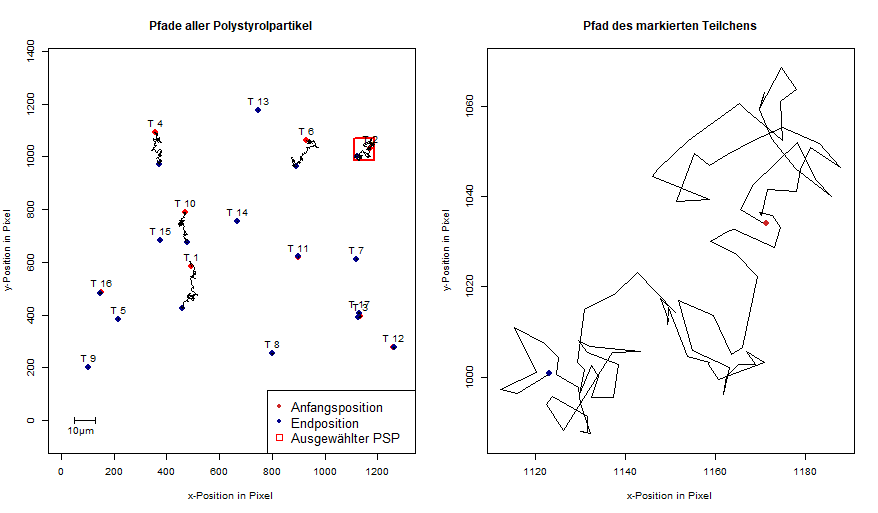
\includegraphics[width=\textwidth,height=0.99\textheight]{code/Plots/Raum.png}
\caption{Auf diesen zwei Plots sind die Positionen aller bzw. eines
markierten PSP im zeitlichen Verlauf zu sehen. Die Aufnahmedauer betrug
100 s mit 1 fps.}
\end{figure}

\hypertarget{auswertung}{%
\subsection{Auswertung}\label{auswertung}}

\hypertarget{interpretation}{%
\subsection{Interpretation}\label{interpretation}}

\end{document}
